% =========================================================================
%  M.Sc research proposal -- Adam Celermajer, Bar-Ilan University
%
%  OVERLEAF: set  Menu -> Compiler -> XeLaTeX  (required for the Hebrew
%  title page). The bundled latexmkrc also selects XeLaTeX.
%  Bibliography: BibTeX with natbib (plainnat), file refs.bib.
%
%  Main study: rule learning from image and grid observations.
%  Section order follows the department template: Introduction, Related
%  Work, Research Goal and Hypotheses, Initial Results, Work Plan, References.
% =========================================================================
\documentclass[11pt,a4paper]{article}

\usepackage[margin=2.5cm]{geometry}
\usepackage{fontspec}
\usepackage{amsmath,amssymb}
\usepackage{booktabs}
\usepackage{array}
\usepackage{tabularx}
\usepackage{graphicx}
\usepackage{xcolor}
\usepackage{enumitem}
\usepackage{caption}
\usepackage[round]{natbib}
\usepackage{microtype}
\usepackage{xurl}
\usepackage{hyperref}

% Polyglossia must come after hyperref (it loads bidi for Hebrew).
\usepackage{polyglossia}
\setdefaultlanguage{english}
\setotherlanguage{hebrew}

% Hebrew font: Culmus fonts are installed on Overleaf. The fallbacks let the
% file also compile on machines without them.
\IfFontExistsTF{David CLM}{%
  \newfontfamily\hebrewfont[Script=Hebrew]{David CLM}}{%
\IfFontExistsTF{Frank Ruehl CLM}{%
  \newfontfamily\hebrewfont[Script=Hebrew]{Frank Ruehl CLM}}{%
\IfFontExistsTF{Noto Serif Hebrew}{%
  \newfontfamily\hebrewfont[Script=Hebrew]{Noto Serif Hebrew}}{%
  \newfontfamily\hebrewfont[Script=Hebrew]{David}}}}

\definecolor{biugreen}{HTML}{005336}
\hypersetup{colorlinks=true,linkcolor=biugreen,citecolor=biugreen,urlcolor=biugreen}

\setlist{itemsep=1pt,topsep=3pt,parsep=0pt}
\captionsetup{font=small,labelfont=bf}
\setcounter{tocdepth}{2} % sections and subsections only; keeps the contents to one page
\setlength{\parskip}{3pt}
\newcolumntype{L}[1]{>{\raggedright\arraybackslash}p{#1}}
\newcolumntype{Y}{>{\raggedright\arraybackslash}X}

\newcommand{\qsmall}{Qwen~3.8-27B}

\begin{document}

% -------------------------------------------------------------------------
% Title page
% -------------------------------------------------------------------------
\begin{titlepage}
  \pagenumbering{gobble}
  \centering
  
\includegraphics[width=0.13\textwidth]{figures/biu-cs-logo.png}\\[0.6cm]
  {\scshape\Large Bar-Ilan University\par}
  \vspace{0.15cm}
  {\Large\texthebrew{אוניברסיטת בר-אילן}\par}
  \vspace{0.6cm}
  {\scshape\large M.Sc.\ Research Proposal\par}
  \vspace{0.1cm}
  {\large\texthebrew{הצעת מחקר לתואר שני}\par}
  \vspace{0.4cm}
  \rule{\linewidth}{0.5pt}\\[0.3cm]
  {\LARGE\bfseries Rule Learning with Small Language Models\\[0.15cm]
   \Large in Interactive Puzzle Games\par}
  \vspace{0.4cm}
  \begin{hebrew}
    {\Large\bfseries למידת חוקי משחק באמצעות מודלי שפה קטנים\par}
    \vspace{0.1cm}
    {\large\bfseries במשחקי חידה אינטראקטיביים\par}
  \end{hebrew}
  \rule{\linewidth}{0.5pt}\\[1.0cm]

  \begin{minipage}[t]{0.45\textwidth}
    \raggedright\large
    \emph{Student:} \texthebrew{סטודנט}\\
    Adam Celermajer\\
    \texthebrew{אדם סלרמאג'ר}
  \end{minipage}\hfill
  \begin{minipage}[t]{0.45\textwidth}
    \raggedleft\large
    % TODO(Adam): confirm both supervisors in writing before submission
    % (if a single supervisor remains, change to "Supervisor:" / מנחה).
    \emph{Supervisors:} \texthebrew{מנחים}\\
    Prof.\ Gal Kaminka\\
    Prof.\ Yoav Goldberg
  \end{minipage}

  \vfill
  {\large Department of Computer Science and Artificial Intelligence\par}
  {\large\texthebrew{המחלקה למדעי המחשב ובינה מלאכותית}\par}
  {\large Bar-Ilan University, Ramat Gan, Israel\par}
  \vspace{0.8cm}
  {\large October 2026\par}
\end{titlepage}

% -------------------------------------------------------------------------
\pagenumbering{roman}
\tableofcontents
\clearpage
\pagenumbering{arabic}
\setcounter{page}{1}
% -------------------------------------------------------------------------

\section{Introduction}
\label{sec:intro}

\textbf{This thesis will enable a small language model to learn game rules
from images, grid observations and interaction, and use those rules to solve
interactive puzzles.} Our primary
target is \qsmall{}. The deliverable is a working agent that discovers the
controls, goal and mechanics of a new game, constructs a useful world model,
and produces solutions that succeed when executed independently. We will use
controlled experiments to identify the capabilities the harness must support
and demonstrate the resulting improvement on games held out from development.

The task is more demanding than solving a puzzle with stated rules. In our
main game-playing conditions, the agent has access to both rendered PNG images
and integer grid observations, together with anonymous action identifiers.
Images provide visual evidence about objects, terrain and targets; they do not
state the transition rules, action meanings or win condition. The agent must
combine visual and symbolic evidence, design informative
experiments, infer what counts as success, and plan with incomplete knowledge.
Later levels test whether the learned rules survive changes in layout and
combinations of mechanics. This is the skill-acquisition setting motivating
ARC-AGI-3 \citep{arcprize2026arcagi3,chollet2019measure}.

The research foundation exists: an ARC-compatible PuzzleScript environment,
diagnostic evaluation artifacts, persistent direct-play baselines, an isolated
adaptation of Agentic Variation Operators (AVO) \citep{chen2026avo}, and a
workbench that traces a solver's result back to the observations, experiments
and revisions that produced it (Section~\ref{sec:results}).

The existing results establish both feasibility and a concrete research target.
AVO-generated solvers have completed all levels of Modality, Knightoban and
IceCrates in fresh environments, including solvers produced by DeepSeek
V4.1 Flash, and a single Qwen~3.8 Max campaign completed Modality. In
contrast, the completed \qsmall{} direct-play pilot achieved 0/4, 0/6 and 3/6
levels on those games, and under AVO it reached 2/4 on Modality with a solver
that misread its own observations. Its recorded behavior reveals specific
failures in action interpretation, goal recognition and hypothesis revision.
Every comparative number so far is a single run. We will close this gap by
turning those diagnoses into tested components of a small-model learning
system, with repeated runs on one fixed harness.

\section{Related Work}
\label{sec:related}

\paragraph{Interactive skill acquisition.}
ARC-AGI-3 evaluates learning through interaction with unfamiliar environments,
including exploration, goal inference and planning
\citep{arcprize2026arcagi3}. PuzzleJAX establishes PuzzleScript as a source of
diverse reasoning and learning tasks \citep{earle2025puzzlejax}. Our platform
retains the original engine as the transition authority and exposes an
ARC-compatible interface. This lets us study how an agent acquires mechanics
while separately measuring predictive knowledge and executable solutions.
The experiments proposed here concern PuzzleScript tasks; they do not claim
a score on the official ARC-AGI-3 benchmark.

\paragraph{Learning game dynamics from interaction.}
Theory-based reinforcement learning shows that an agent which induces an
explicit theory of objects, rules and goals and plans with it reaches
human-like sample efficiency on novel video games \citep{tsividis2021theory}.
Program-synthesis world models extend this to language models:
WorldCoder \citep{tang2024worldcoder} writes and repairs a Python transition
model from interaction, code world models guided by Monte Carlo tree search
\citep{dainese2024codeworldmodels} select among candidate programs by their
predictions, and PoE-World \citep{piriyakulkij2025poeworld} composes many
small programmatic experts into a model of Atari-style games from a few
demonstrations. All of these use frontier models as the program writer. We
share the executable-model representation but target a fixed small model
and ask which capability prevents it from learning.

\paragraph{Hypothesis formation and revision in language models.}
Language models propose and refine hypotheses well when the loop is
externally structured: Hypothesis Search generates natural-language rules
for ARC tasks, turns them into programs and keeps those that pass the
examples \citep{wang2024hypothesissearch}. They do poorly when asked to
find a rule and then apply it themselves: iterative refinement improves
the proposals, but the models remain weak at executing their own rules
\citep{qiu2024phenomenal}. Our 27B traces show the second pattern: a wrong
explanation of an accidental win is retained across levels. The proposed
experiment-and-revision components target exactly this.

\paragraph{Agent interfaces and persistent learning.}
ReAct interleaves reasoning and actions to support grounded decision making
\citep{yao2023react}. SWE-agent demonstrates that the interface provided to a
language model affects its ability to carry out a task
\citep{yang2024sweagent}. Reflexion and Voyager add verbal self-revision and
a persistent skill library across episodes
\citep{shinn2023reflexion,wang2023voyager}. We investigate this principle
under a different constraint: the model must learn the task's mechanics and
objective rather than follow a stated specification. Our direct-play and
coding-agent runners provide an existing basis for controlled comparisons of
memory, tools, observation formats and experiment structure.

\paragraph{Executable models and evolutionary improvement.}
FunSearch evolves programs scored by an external evaluator
\citep{romeraparedes2024funsearch}. AVO replaces the sampled mutation with
autonomous coding agents as variation operators that propose and improve
implementations with execution feedback \citep{chen2026avo}; the
same architecture has been reported to solve ARC-AGI-3 with frontier models
\citep{nvidia2026avoarc}, and RSIAgent studies autonomous exploration for
self-improvement in new environments \citep{zhu2026rsiagent}. Our adaptation
combines game research, strategy evolution and a separate fresh-solver
evaluation. This creates a testable connection between a model's hypotheses
and an executable artifact: a candidate earns its score only when its solver
succeeds independently.

\paragraph{Benchmarks for agents in games.}
BALROG \citep{paglieri2025balrog} and SmartPlay \citep{wu2024smartplay}
evaluate language agents on long-horizon games with stated rules and
report that vision-based variants lag their text counterparts; Baba Is AI
\citep{cloos2024baba} requires agents to manipulate the rules themselves
and finds failures when rules must be combined; WorldTest
\citep{warrier2026worldtest} separates an interaction phase from queries
about the learned world model. PuzzleJAX \citep{earle2025puzzlejax} and
ARC-AGI-3 supply unknown rules.
Unlike these, our platform scores a learned rule against the game source
by replaying counterfactual actions in the real engine, separating rule
accuracy from task success.

\paragraph{Harness effects and format sensitivity.}
Interface choices change what a model can do: enforced output formats
degrade reasoning \citep{tam2024letmespeak}, prompt formatting changes
scores by many points \citep{sclar2024quantifying}, and visual harnesses
alter agent behaviour \citep{han2026vista}. Agent evaluations must also
control cost \citep{kapoor2024agents}. Our JSON-schema diagnostic is an
instance of the first effect; our resource reporting follows the last.

\paragraph{Scale and measurement.}
Scaling laws describe loss, not task competence \citep{kaplan2020scaling},
and abilities that appear to emerge abruptly with scale
\citep{wei2022emergent} can be artefacts of discontinuous metrics
\citep{schaeffer2023mirage}. Whether a 27B model ``can'' learn a game
therefore depends on how learning is measured. We use graded measures,
levels completed and counterfactual rule accuracy, rather than a binary
solved flag, and we do not treat a difference between Qwen~3.8 sizes as a
scale effect without the controls in Section~\ref{sec:plan}.

\paragraph{Prior knowledge, small open models and training exposure.}
Human game learning depends partly on object and game conventions
\citep{dubey2018priors}. Our traces suggest that recognizing conventions such
as undo and box pushing can simplify discovery substantially. However,
whether a model has seen similar environments cannot be read off its
behaviour; contamination studies \citep{golchin2024timetravel,elazar2024wimbd}
show how hard attribution is even with open corpora. We therefore treat
pretraining as a bounded, not identified, factor (Section~\ref{sec:goal}),
and test whether explicit exploration and verification allow the 27B model
to acquire the missing knowledge during play.

\paragraph{Position.}
The contribution is not another world-model agent. It is (i) a
capability-level diagnosis of \emph{why} a fixed small open model fails,
with rule accuracy audited against the game source by counterfactual replay;
(ii) controlled interventions that supply ground truth as diagnostics; and
(iii) an evaluation that separates rule accuracy from winning.

\section{Research Goal and Hypotheses}
\label{sec:goal}

\subsection{The task}

PuzzleScript is a language for turn-based grid games
\citep{lavelle2013puzzlescript}. A game defines objects and their appearance,
rewrite rules for state transitions, a win condition, and an ordered sequence
of levels. The resulting tasks include box-pushing puzzles, sliding motion,
objects with different movement rules, mode changes, and interactions whose
effects depend on terrain or history. Their compact appearance makes the
mechanics inspectable by an evaluator while leaving substantial discovery
and planning work for an agent.

Our collection contains 206 game entries; experiments use curated, versioned
playable subsets. The agent sees neither the game identity nor the source.
The encoding \texttt{visible-cell-v1} assigns an anonymous integer to each
rendered tile texture; the direct player receives the rendered PNG alongside
the grid at each turn, and AVO exposes rendered observations through its
research interface. Object-name legends and action meanings are withheld.
Identical visible textures may conceal different underlying states, so the
agent may need observation history rather than a transition model based on
the latest frame alone.

\subsection{Example: Modality}

Figure~\ref{fig:modality} illustrates the distinction between seeing a board
and understanding a game. In Modality, the player cannot move directly between
white and black terrain; a checkered tile connects them. Crate pushing depends
on compatible terrain, the goal is to place crates on targets, and
\texttt{ACTION7} undoes a move. None of this is stated: calling undo a jump
changes the interpretation of earlier transitions, and calling a crate the
goal sends plans toward the wrong objective.

\begin{figure}[ht]
  \centering
  \begin{minipage}[c]{0.29\textwidth}\centering
    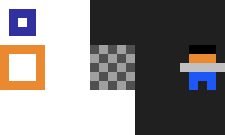
\includegraphics[width=\linewidth]{figures/modality-level1.png}\\
    {\small (a) First-level image}
  \end{minipage}\hspace{0.6cm}
  \begin{minipage}[c]{0.21\textwidth}\centering
    {\small\ttfamily\begin{tabular}{@{}ccccc@{}}
      0&1&2&2&2\\ 3&1&4&2&5\\ 1&1&1&2&2
    \end{tabular}}\\[4pt]
    {\small (b) Anonymous tile grid}
  \end{minipage}\hspace{0.6cm}
  \begin{minipage}[c]{0.24\textwidth}\centering
    
\includegraphics[width=\linewidth]{figures/modality-level2.png}\\
    {\small (c) A later layout}
  \end{minipage}
  \caption{Modality observations. For the evaluator, the initial IDs denote a
  target (0), white floor (1), black floor (2), crate (3), bridge (4) and player
  on black floor (5). These meanings are not supplied to the agent. Later
  levels require reusing the inferred mechanics on new configurations.}
  \label{fig:modality}
\end{figure}

\subsection{Capabilities}

We decompose the task into the seven capabilities in
Table~\ref{tab:challenge}. The decomposition connects the experimental
measurements to concrete design decisions. It also distinguishes a failure
to learn a game from a failure of the software protocol.

\begin{table}[ht]
  \centering\small
  \begin{tabularx}{\linewidth}{L{0.17\linewidth} Y Y}
    \toprule
    Capability & Required behavior & Diagnostic evidence \\
    \midrule
    Perception & Ground objects in images and grids; track changing textures and hidden state. &
    Object tracking and next-frame predictions. \\
    Action interpretation & Discover movements, undo, selection and commitment. &
    Controlled action tests and the agent's stated control model. \\
    Rule induction & Learn conditional effects, including interactions. &
    Predicted versus observed transitions; tests distinguishing rival rules. \\
    Goal recognition & Infer the actual win condition. &
    Goal statements and hidden, elicited and supplied-goal conditions. \\
    Planning & Find legal solutions and recover from dead ends. &
    Fresh solver evaluations, search traces and recovery actions. \\
    Transfer & Reuse and refine knowledge across levels. &
    Performance when familiar mechanics appear in new layouts. \\
    Credit assignment & Explain why an action sequence produced a win. &
    Post-win reconstruction checked against the winning transition. \\
    \bottomrule
  \end{tabularx}
  \caption{Capabilities supporting rule learning and its use in planning.}
  \label{tab:challenge}
\end{table}

These capabilities interact. A wrong goal can invalidate a correct movement
model; an incorrect interpretation of undo can make a recoverable planning
error appear permanent. The proposed agent will maintain explicit links
between observations, hypotheses and plans so that contradictory evidence
causes a revision rather than a new local explanation for every failure.

\subsection{Objective}

\textbf{We will build a small-model rule-learning agent that infers game
dynamics from image and grid transitions and produces working puzzle
solutions.} \qsmall{} is the primary
development model. We will keep its weights fixed while developing the
harness, so improvements can be attributed to the agent system. Larger
models provide diagnostic comparisons and successful learning traces; the
final small-model condition will not rely on a larger model selecting its
actions or revising its solver at evaluation time. The thesis therefore
manipulates one factor, the harness, with the model fixed; model size and
pretraining exposure are bounded by controls, not identified.

The harness will support a complete learning cycle: formulate a hypothesis,
choose a discriminating experiment, compare a predicted transition with the
real outcome, revise the world model, and plan using the verified knowledge.
Memory will retain the evidence for a rule and its unresolved cases, not only
a conclusion. In the coding condition, learned knowledge will be converted
into a solver that is tested from a fresh reset.

Three research questions guide construction:
\begin{enumerate}[leftmargin=1.5em]
  \item Which capabilities distinguish correct rule acquisition and revision
  from the observed failures of the small model?
  \item Which of these capabilities can be supplied or strengthened through
  exploration, memory, verification and planning support?
  \item Do the learned rules predict held-out transitions and support reliable
  puzzle solutions, including on games held out from harness development?
\end{enumerate}

\paragraph{Testable hypotheses.}
\begin{description}[leftmargin=1.2em]
  \item[H1: Learning structure.] An explicit experiment-and-revision loop
  improves rule prediction and whole-game success over the direct-play baseline with
  the same small model and provider.
  \item[H2: Goal and control bottlenecks.] Correcting goal recognition or
  action interpretation removes a substantial part of the observed failures.
  Separate interventions will measure which component matters in each game.
  \item[H3: Externalized planning.] Executable world models, deterministic
  search and fresh evaluation improve solution reliability beyond verbal
  planning alone.
  \item[H4: Capability gaps are localisable.] Under one fixed harness, the
  Qwen~3.8 models fail at identifiable stages (observation parsing, action
  interpretation, rule consolidation, verification) rather than uniformly,
  and the stage at which 27B fails is the one whose support most improves
  it. We do not claim to separate parameter count from architecture,
  post-training or serving; a same-size dense model from another family and
  a zero-shot next-frame probe bound, but do not identify, those factors.
\end{description}

\section{Initial Results}
\label{sec:results}

We report results first and the platform that produced them last. Every
comparative number below comes from a single run per model and condition.

\subsection{Pilot: the Qwen 3.8 family on Modality (single runs)}

Table~\ref{tab:family} reports one run per model and condition on Modality,
all with high reasoning effort and first-party Alibaba routing. Baseline+ is
direct play with note tools and a 100-action budget; AVO allows 300 research
actions, two real solver self-checks and a 1,500-action final evaluation of a
frozen solver. The conditions are not resource-matched and each cell is a
single run; the table motivates the comparisons in the Work Plan rather than
establishing a ranking. Every recorded action (3,700 across eight logs) was
replayed in the native PuzzleScript engine with no position or level mismatch.

\begin{table}[ht]
  \centering\small
  \begin{tabular}{lcccr}
    \toprule
    Model & Baseline+ (100 actions) & AVO research & AVO final solver & Solver actions \\
    \midrule
    Qwen 3.8 Max   & 1/4 & 3/4 (123 actions) & \textbf{4/4} & 265 \\
    Qwen 3.8 Flash & 1/4 & 3/4 (160 actions) & 1/4 & 1,500 \\
    Qwen 3.8-27B   & 0/4 & 1/4 (234 actions) & 2/4 & 1,500 \\
    \bottomrule
  \end{tabular}
  \caption{Modality, October 2026, $n=1$ per cell. The three baseline+ runs
  share harness, provider, effort, budget and observation format (the 27B run
  is five days older). Flash is a 125B mixture-of-experts model with 6B active
  parameters; 27B is dense. Level 4 was visible to Max during research, so the
  4/4 is not a held-out result. The harness used has since been retired
  (Section~\ref{sec:plan}).}
  \label{tab:family}
\end{table}

Three verified observations shape the proposal. First, winning did not
require a correct rule: Max's solver models the checkered tile as a global
phase toggle and exempts target cells from the terrain test, and
counterfactual replay in the real engine finds 32 wrong predictions among
1,060 alternative moves at its own decision states (27 too strict, 5 too
permissive); none of those situations arose on its 265-action path. Second,
Flash's research planner encoded the exact player-movement rule (no direct
move between white and black floor, though not the push rule) and used it
to clear levels 2--3, but never wrote it into its notes or world model; its
final solver relearned the same movement rule online within 80 actions and
still spent 1,490 actions oscillating on level 2, so the cause of its 1/4 is
open. Third, 27B's solver parsed the older of the two
frames in each observation, built delayed-action mechanics that fit its own
misreading, and chose a position no-op in 1,405 of its 1,420 level-3
actions; in direct play it read undo as a ``jump'' and declared a recoverable
deadlock permanent. These are recorded behaviours, not demonstrated causes;
isolating causes is the first stage of the Work Plan.

\subsection{The 27B direct-play gap across games}

The \qsmall{} direct-play pilot (Table~\ref{tab:qwen}) used the same
condition on three games: baseline+ through the Codex harness routed to
OpenRouter, Alibaba provider, high effort, image and grid observations.
Each run reached its action budget, so the partial IceCrates result is
directly distinguishable from a startup or transport error.

\begin{table}[ht]
  \centering\small
  \begin{tabular}{lrrll}
    \toprule
    Game & Budget & Levels & Harness / provider & Evidence for the next intervention \\
    \midrule
    Modality & 100 & 0/4 & Codex / Alibaba & Undo misread; crate deadlock not recovered \\
    Knightoban & 120 & 0/6 & Codex / Alibaba & Goal and special movement not identified \\
    IceCrates & 120 & 3/6 & Codex / Alibaba & Undo identified; later mechanics unresolved \\
    \bottomrule
  \end{tabular}
  \caption{Completed 27B direct-play pilot, October 2026, one run per game
  ($n=1$), all on the Codex harness via OpenRouter with the Alibaba provider.
  AVO and direct-play results are distinct conditions; their difference
  motivates, rather than replaces, matched comparisons.}
  \label{tab:qwen}
\end{table}

In IceCrates the same model identified undo and solved three levels in its
first 27 actions, so the research target is the reliable acquisition and
revision of specific mechanics, not an assumption that the model has no
game-playing ability. We have also isolated one interface effect: in a small
controlled diagnostic, an enforced JSON action schema yielded zero note-tool
calls in two checks, whereas the corresponding checks without that schema
each called the tool. The action parser now accepts valid actions surrounded
by prose and requests a correction for unusable replies; provider pinning and
recorded request metadata reduce routing ambiguity. These checks are reported
separately from game-learning outcomes.

\subsection{Whole-game solving and mechanics recovery by larger models}

Table~\ref{tab:success} reports representative best fresh evaluations. These
are independently executed solvers, not scores inferred from research notes
or from the model's claim that it has understood a game.

\begin{table}[ht]
  \centering\small
  \begin{tabular}{llrr}
    \toprule
    Game & Player / optimizer & Levels & Solver actions \\
    \midrule
    Modality & GPT-5.6 Luna / GPT-6 Astra & 4/4 & 263 \\
    Knightoban & GPT-5.6 Luna / GPT-6 Astra & 6/6 & 255 \\
    IceCrates & GPT-6 Astra / GPT-6 Astra & 6/6 & 138 \\
    Modality & DeepSeek V4.1 Flash / same & 4/4 & 263 \\
    Knightoban & DeepSeek V4.1 Flash / same & 6/6 & 216 \\
    IceCrates & DeepSeek V4.1 Flash / same & 6/6 & 90 \\
    \bottomrule
  \end{tabular}
  \caption{Observed AVO whole-game successes. Rows report the best completed
  fresh evaluation from the corresponding campaign, not averages across
  repeated attempts ($n=1$ per row). Model-role settings are retained in the
  run manifests.}
  \label{tab:success}
\end{table}

We audited the discovered mechanics against the source rules after the runs.
In Modality, controlled tests established terrain-dependent movement and
pushing. In Knightoban, the agent separated move preview, spatial selection
and action-key commitment and constructed a planner for interacting pieces.
In IceCrates, experiments distinguished moving crates from walls, established
water filling and the need to stop on the goal, and corrected a missing rule
for pushing a two-crate train; after that correction, the independent solver
completed all six levels. The audit relies on contemporaneous strategies,
transitions and solver code and establishes the mechanics needed by the
successful solvers, not that every unobserved combination was characterized.
GPT-5.6 Luna also solved Feeling Like Filling (6/6), Mowing (4/4) and
Fatigued Square Maze (8/8) in both recorded repeats of the six-game
comparison, and Enqueue reached 8/14 levels with both the GPT-6 Luna and
DeepSeek Flash configurations. These supply successes and partial-progress
cases for testing whether small-model improvements transfer across mechanics.

\subsection{Goal-recognition data}

We also completed data collection for a separate goal-recognition study.
Four models (Claude Opus~4.8, GPT-5.5, Kimi~K2.6 and DeepSeek~V4~Pro)
described the goal and win condition of 50 curated games from an initial
frame or an initial frame followed by three random actions, in text or
text-plus-image conditions (700 predictions); 38 human participants gave 114
goal descriptions across 48 games. Correctness annotation has not started,
so no accuracy is claimed. The collection exposed a representation confound:
initial-frame text prompts used game-specific glyphs while trajectory prompts
used anonymous IDs, and a model read \texttt{@} as a player when it denoted a
crate on a target. The Work Plan bounds the analysis to one condition with
this difference explicit.

\subsection{The platform that produced these results}

The implementation separates the game engine from the agent interface. A
Node.js runtime executes the PuzzleScript rules; a Python service adapts it
to the ARC interaction contract, including resets, actions and scorecards,
and the same agent code can address an official ARC backend. Evaluator
artifacts measure knowledge independently of winning: the benchmark set
covers 21 games with replay-verified reference trajectories and ten unique
next-observation probes per game, scored by exact-frame accuracy, cell
accuracy and transition-edit measures; no model has been scored on it yet.
The workbench records settings, process ownership, frames, transitions, note
revisions, model requests and solver files for every run, and replays any
action with the reasoning that produced it.

An earlier explicit rule-induction agent records state--action--state
transitions, asks a model to propose rules, compiles them into an executable
logical form and checks them against the evidence; its saved Sokoban
experiments hold verified movement, collision and crate-push rules, and it is
the baseline representation for the proposed learning cycle.

\paragraph{Direct play.}
The direct player maintains one model session across the game. The baseline+
condition adds persistent note tools and a strategy file while retaining the
same action and observation loop, with recorded transitions and immutable
note revisions.

\paragraph{AVO adaptation.}
We implemented a distinct research--optimization--evaluation architecture.
An inner coding agent explores the game, compares continuations from saved
checkpoints and constructs a solver; an outer optimizer improves strategies
through a recorded candidate lineage; a trusted evaluator then executes each
frozen solver from a fresh reset, without language-model calls. The
candidate's fitness is the number of levels completed in this independent
evaluation:
\[
  \text{strategy}_i\ \longrightarrow\ \text{research}_i
  \longrightarrow\ \texttt{solver}_i
  \longrightarrow\ \text{fresh evaluation}.
\]
Model commands run in a sandbox without access to game sources, evaluation
artifacts or the network; the trusted controller owns environment and
provider communication and retains strategies, feedback and world-model
reports, whose presence does not affect fitness.

\section{Work Plan}
\label{sec:plan}

\subsection{First: compare the Qwen~3.8 family on one fixed harness}

The October pilot (Table~\ref{tab:family}) used a Codex-based harness routed
through OpenRouter that has since been retired. The confirmatory comparison
will fix one harness (the OpenCode or bare runner, chosen and frozen before
the first run), Alibaba routing, high effort, image and grid observations, a
100-action direct-play budget and the AVO budgets above, with three
independent runs per model and game. Harness version is recorded as an
experimental factor and never changed mid-comparison. The same model
occupies the player and optimizer roles in AVO, and direct-play and AVO
outcomes remain separate, with their action, candidate, time and token
budgets reported explicitly.

This experiment identifies the next useful intervention. If Max discovers
the decisive rule but 27B does not, we will compare the experiments and
revisions that led to it. If the same smaller model succeeds under AVO,
we will isolate which support made the difference. If the family stalls on
the same mechanic, we will target that shared bottleneck. Family differences
do not isolate parameter count: two controls bound size and pretraining
without identifying them, a dense open model of similar size from another
family on the same harness, and the zero-shot next-frame probe on the
existing 21-game benchmark. The comparison covers Modality, Knightoban and
IceCrates, which supply distinct challenges in terrain, selection and
commitment, and multi-object sliding interactions.

\subsection{Second: locate the bottleneck through controlled interventions}

We will use the capability decomposition to select interventions, rather
than add several forms of assistance at once. Initial conditions will test:
\begin{enumerate}[leftmargin=1.5em]
  \item \textbf{Goal recognition:} the goal is hidden, explicitly elicited
  and revised, or supplied by the evaluator.
  \item \textbf{Action interpretation:} controls remain anonymous, or their
  true meanings are supplied while the rules and goal remain hidden.
  \item \textbf{Mechanics and planning:} selected true mechanics are supplied
  diagnostically, or the model's learned mechanics are paired with a
  deterministic planner.
\end{enumerate}
Supplying the truth is a diagnostic intervention, not the final task setting.
A gain under a supplied-goal condition estimates how much incorrect goals
contribute to failure; a residual gap motivates further tests of dynamics
and planning. The final agent must acquire the hidden information itself.

For each failed attempt we will identify the first consequential mismatch
between the model's belief and the observed transition, along with secondary
causes such as failure to recover. Annotators will cite the supporting step,
action and note rather than infer the cause from terminal reward alone.
Independent human annotation of a sample will assess the reliability of the
taxonomy; we will report agreement and disagreements rather than treat an
automatic label as ground truth.

The goal-recognition corpus is a bounded side task: annotate the
initial-frame condition (50 games, four models) against the game win
conditions with a correct/partial/incorrect rubric and report model--human
agreement with the representation difference explicit.

\subsection{Third: build and ablate the support that makes the small model solve}

We will develop the harness from the diagnosed failures. Candidate components
are a ledger linking hypotheses to evidence, controlled experiment selection,
explicit transition predictions, revision when evidence contradicts a rule,
and reconstruction of what caused each win. The ledger
will distinguish observed, predicted and untested cases, preserving uncertainty
instead of recording unknown moves as walls or no-ops.

The coding condition will support executable world models and search. The
small model will infer and implement the mechanics; deterministic procedures
will handle repeated simulation and path search. A mismatch between simulation
and a real transition will invalidate the relevant rule or plan and trigger
new research. Fresh solver evaluation will verify that the resulting program
works without continued language-model guidance.

Each component will first be compared with the established baseline under
matched conditions. We will then combine components that produce repeatable
gains and remove them individually to determine their contribution. The
comparison will record the actual observation history, context policy and
tool inventory, since changing these silently can change the task.

\subsection{Validation, efficiency and generalization}

Let $L(m,h,g)$ be the number of levels completed by model $m$ with harness
$h$ on game $g$, and let $n_g$ be the number of playable levels. Two
outcomes are primary: $L/n_g$ on held-out layouts, and counterfactual rule
accuracy $A(m,h,g)$: for each recorded decision state the real engine is
restored and all legal actions are executed; $A$ is the fraction the learned
model predicts correctly. Every table reports both, so that a win obtained
with a wrong model (as in the Max pilot) is visible. We will also report
whole-game success, actions, candidate evaluations, elapsed search time,
tokens and measured API cost. For AVO, the solver outcome comes from the
fresh frozen solver; research progress is an additional diagnostic.
Next-observation accuracy and goal correctness measure learned knowledge
separately from task completion.

Development uses the three diagnostic games. Before final evaluation, we
will select and freeze a held-out subset from the curated collection,
covering different mechanics and level structures. Game sources, verified
solutions and source-derived annotations remain evaluator-only. Runs are
independent, and no notes or solutions from a held-out game are inherited
by its evaluated agent. We will report repeated-attempt outcomes as counts
($k/n$ solved, median levels) and uncertainty, not only the best candidate.

The primary success criterion is that the fixed small model learns rule models
that predict held-out transitions and enable complete solutions on games its
baseline fails, with repeatable gains under declared resource budgets.
A solver that improves only on a development
layout is an intermediate result; the final contribution must demonstrate
that the learning procedure transfers.

\subsection{Timeline, deliverables and resources}

Table~\ref{tab:milestones} defines the remaining work by stage, with months,
run counts and estimated cost. Family-comparison results will guide the
interventions, with repeated experiments concentrated on promising conditions.

% TODO(Adam): adjust the months to the actual thesis deadline and confirm the
% cost estimates (list prices, no billing data) before submission.
\begin{table}[ht]
  \centering\small
  \begin{tabularx}{\linewidth}{L{0.16\linewidth} Y L{0.13\linewidth} r r}
    \toprule
    Stage & Work and completion evidence & Months & Runs & Est.\ cost \\
    \midrule
    Family comparison & Freeze one harness; 3 models $\times$ 3 games
    $\times$ \{baseline+, AVO\} $\times$ 3 repeats, plus the two bounding
    controls. Evidence: matched settings, outcomes, rule accuracy, costs and
    decisive-rule trace comparisons. & Nov--Dec 2026 & 54 & $\approx$\$700 \\
    Bottleneck analysis & Interventions on 27B and Flash: supplied goal,
    supplied actions, latest-frame-only observation, enforced self-check,
    rival-hypothesis step; 3 repeats plus controls. Evidence: scored
    interventions, annotated failure traces with agreement, bounded
    goal-corpus analysis. & Jan--Mar 2027 & $\approx$90 & $\approx$\$400 \\
    Small-model solver & Implement and combine experiment, memory,
    verification and search support; ablations on the development games.
    Evidence: whole-game successes by the fixed small model; component
    ablations. & Apr--Jun 2027 & $\approx$60 & $\approx$\$300 \\
    Generalization & Freeze the harness and held-out games; 6 games
    $\times$ 3 repeats $\times$ \{baseline, harness\}. Evidence: fresh solver
    scores, rule accuracy, uncertainty and efficiency comparisons. &
    Jul--Aug 2027 & 36 & $\approx$\$200 \\
    Thesis and release & Document the method, artifacts and limits.
    Evidence: reproducible implementation, experiment records and thesis. &
    Sep--Oct 2027 & --- & --- \\
    \bottomrule
  \end{tabularx}
  \caption{Timeline for the remaining research. Run counts are planned
  campaigns or direct-play runs. Costs are list-price estimates with no
  billing data behind them; Max dominates the first stage.}
  \label{tab:milestones}
\end{table}

\paragraph{Resource management.}
We will enforce action, candidate and wall-time budgets, record tokens and
measured costs, and retain unsuccessful attempts. Infrastructure errors will
be distinguished from capability outcomes. All requests are recorded with
model id, provider, effort and usage; the 27B model is open-weights and can
be served locally for the final evaluation, while Max is a diagnostic
comparator only.

\paragraph{Expected contributions.}
We will deliver a working rule-learning agent built around a small model,
validated on held-out games by rule accuracy and whole-game success. The
research will also provide a validated capability taxonomy, scored
goal-recognition data, component ablations, and reproducible rule-prediction
and fresh-solver evaluations.

\clearpage
\phantomsection
\addcontentsline{toc}{section}{References}
\bibliographystyle{plainnat}
\bibliography{refs}
\end{document}
